\begin{frame}
    \titlepage
\end{frame}

{
\setbeamercolor{background canvas}{bg=blue!40!black,fg=blue!10!white}
\setbeamercolor{normal text}{bg=blue!40!black,fg=blue!10!white}
\setbeamercolor{itemize/enumerate body}{fg=white}
\setbeamercolor{itemize/enumerate subbody}{fg=white}
\setbeamercolor{titlelike}{bg=blue!40!black,fg=blue!10!white}
\begin{frame}<1|handout:1>[noframenumbering]{Changelog}
    \begin{itemize}
        \item Corrections made in this version not in first posting:
        \begin{itemize}
        \item 28 Feb 2017: slide 55: REX prefix's first nibble is {\tt 0100}
        \end{itemize}
    \end{itemize}
\end{frame}
}

\begin{frame}{VM assignment}
    \begin{itemize}
    \item please do it if you haven't
    \end{itemize}
\end{frame}

\begin{frame}{RE assignment}
    \begin{itemize}
    \item assembly reading practice
    \end{itemize}
\end{frame}

\begin{frame}{example manual page}
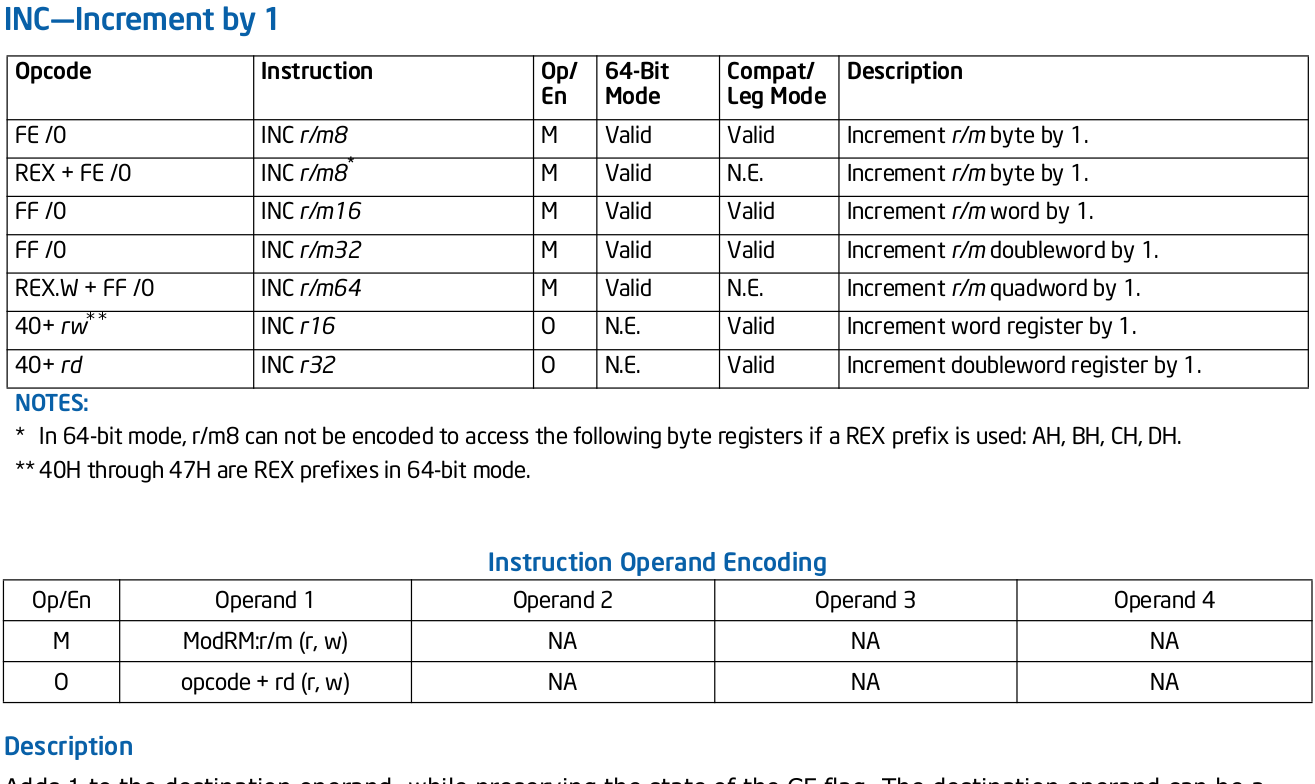
\includegraphics[width=\textwidth]{example-manual}
\end{frame}

\begin{frame}{question: what was /0}
    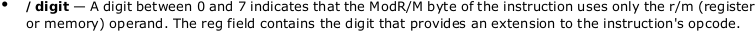
\includegraphics[width=\textwidth]{slashZeroExplain}
    \begin{itemize}
    \item ``{\bfseries / digit} --- A digit between 0 and 7 indicates that the ModR/M byte of the instruction uses only the r/m (register or memory) operand. The {\tt reg} field contains the digit that provides an extension to the instruction's opcode.''
    \item huh? {\tt ModR/M}? later today or Wednesday 
    \end{itemize}
\end{frame}

\begin{frame}[fragile,label=LEA]{LEA}
\lstset{language=myasm}
\begin{itemize}
    \item like a {\tt mov} --- but stop at finding the memory address
    \item \myemph{never} accesses memory
    \item \lstinline|lea (%rax), %rbx| is \lstinline|mov %rax, %rbx|
\end{itemize}
\end{frame}

\begin{frame}[fragile,label=segmentation]{segmentation}
    \begin{itemize}
    \item before virtual memory, there was \myemph{segmentation}
    \end{itemize}
\begin{tikzpicture}
    \tikzset{>=Latex}
    \node[draw,label={north:address},rectangle split,rectangle split parts=2,
        rectangle split horizontal,font=\small,align=left] (address) {
        segment \#: \\ \color{orange!70!black}{\tt 0x1} \nodepart{two} offset: \\ \color{magenta!70!black}{\tt 0x23456}
    };
    \matrix[tight matrix,nodes={text width=2cm,font=\small\tt,text depth=.4ex,text height=1.2ex},
        column 1/.style={nodes={text width=1.5cm}},
        anchor=north west,
        visible on=<1>,
    ] (table) at ([xshift=.5cm]address.north east){
        seg \# \& base \& limit \\
        0 \& 0x14300 \& 0x60000 \\
        |[orange!70!black]| 1 \& |[blue!70!black]| 0x50000 \& |[green!70!black]| 0x6F000 \\
        2 \& 0x70000 \& 0x30000 \\
    };
    \matrix[tight matrix,nodes={text width=2cm,font=\small\tt,text depth=.4ex,text height=1.2ex},
        column 1/.style={nodes={text width=1.5cm}},
        column 3/.style={nodes={font=\scriptsize\tt, text width=6cm}},
        anchor=north west,
        visible on=<2>,
    ] (table2) at ([xshift=.5cm]address.north east){
        seg \# \& base \& limit \\
        0 \& 0x0 \& 0xFFFF FFFF FFFF FFFF \\
        |[orange!70!black]| 1 \& |[blue!70!black]| 0x0 \& |[green!70!black]| 0xFFFF FFFF FFFF FFFF \\
        2 \& 0x0 \& 0xFFFF FFFF FFFF FFFF \\
    };
    \node[draw,circle,font=\large] (plus) at ([yshift=-2cm]address.two south) { $+$ };
    \node[font=\large,draw] (less) at (table-3-3.south |- plus) { $<=$ };
    \draw[magenta!70!black,thick,->] (address.two south) -- (plus);
    \draw[blue!70!black,thick,->] (table-3-2.south) |- (plus);
    \draw[green!70!black,thick,->] ([xshift=.25cm]table-3-3.south) -- ([xshift=.25cm]less.north);
    \draw[magenta!70!black,thick,->] (address.two south) -- ($(plus.north) + (0, .5cm)$) -| ([xshift=-.25cm]less.north);
    \draw[thick,->] (plus) -- ++ (0,-1cm) node[below] { computed address };
    \draw[thick,->] (less) -- ++ (0,-1cm) node[below,align=center] { no segmentation \\ fault?};
\end{tikzpicture}
\end{frame}


\begin{frame}[fragile, label=x86Seg]{x86 segmentation}
\begin{itemize}
\item addresses you've seen are the \myemph{offsets}
\item but every access uses a segment number!
\item segment numbers come from registers
    \begin{itemize}
    \item CS --- code segment number (jump, call, etc.)
    \item SS --- stack segment number (push, pop, etc.)
    \item DS --- data segment number (mov, add, etc.)
    \item ES --- addt'l data segment (string instructions)
    \item FS, GS --- extra segments (never default)
    \end{itemize}
\item instructions can have a \myemph{segment override}:
\begin{lstlisting}
movq $42, %fs:100(%rsi)
    // move 42 to segment (# in FS),
    // offset 100 + RSI 
\end{lstlisting}
\end{itemize}
\end{frame}

\begin{frame}[fragile,label=x86SegPic]
\vspace{-.25cm}
\tikzset{every picture/.style={very thick},every node/.style={fill=white,inner sep=.1mm}}
\begin{tikzpicture}
\node[anchor=north west] at (0,0){
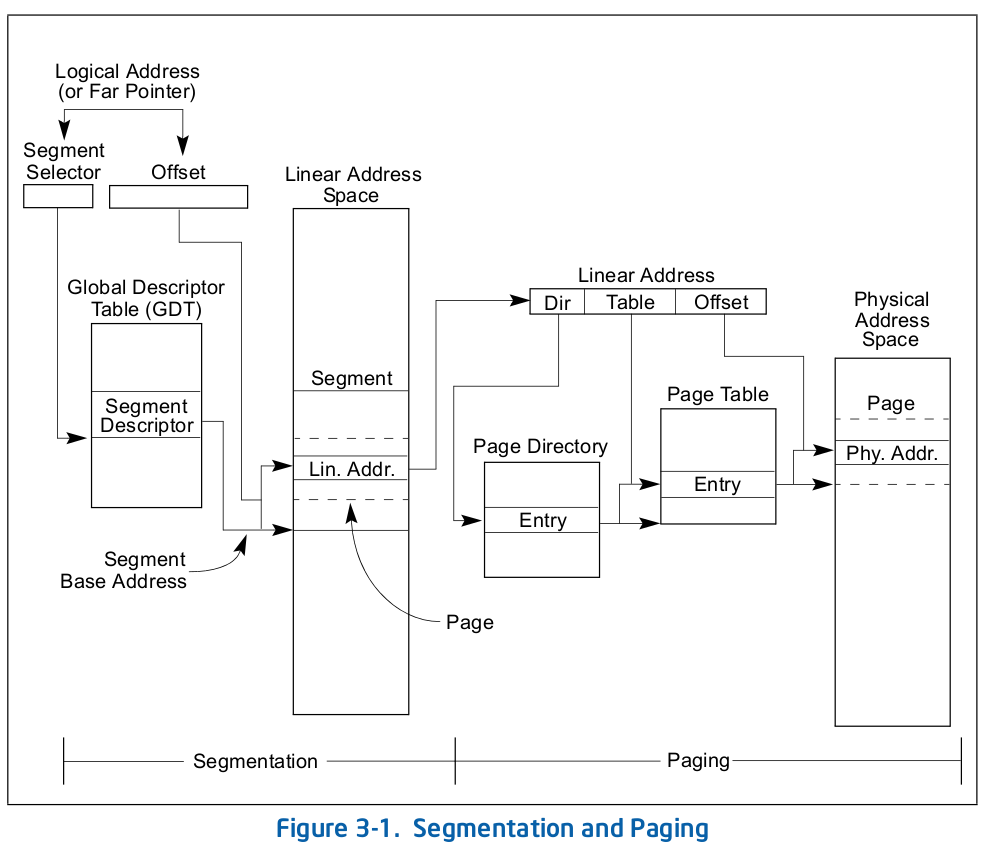
\includegraphics[width=\textwidth]{seg-and-page}
};
%\draw[help lines] (0,0) grid (12, -8);
\begin{visibleenv}<2>
    \draw[blue] (0.8,-0.8) rectangle (2.5,-1.4);
    \node[text=blue!70!black,anchor=south,font=\small] at (1.6,-.8) {program address};
    \draw[green] (6.4,-3.3) rectangle (9.1,-3.9);
    \node[text=green!70!black,anchor=south,font=\small,align=center] at (7.5,-3.3) {after segmentation \\
                                                  ``virtual address''};
    \draw[magenta] (0.9,-3.4) rectangle (2.8,-6.1);
    \node[text=magenta!70!black,anchor=south,font=\small] at (1.8,-3.4) {segment table};
\end{visibleenv}
\begin{visibleenv}<3>
    \draw[red] (0.3,-1.6) rectangle (1.4,-2.4);
    \node[text=red,anchor=west] at (1.4,-2.0) {from instruction + segment register};
\end{visibleenv}
\end{tikzpicture}
\imagecredit{Figure: Intel manuals, Vol 3A}
\end{frame}

\begin{frame}{x86 segment descriptor}
\vspace{-.25cm}
\tikzset{every picture/.style={very thick},every node/.style={fill=white,inner sep=.2mm}}
\begin{tikzpicture}
\node[anchor=north west] at (0,0){
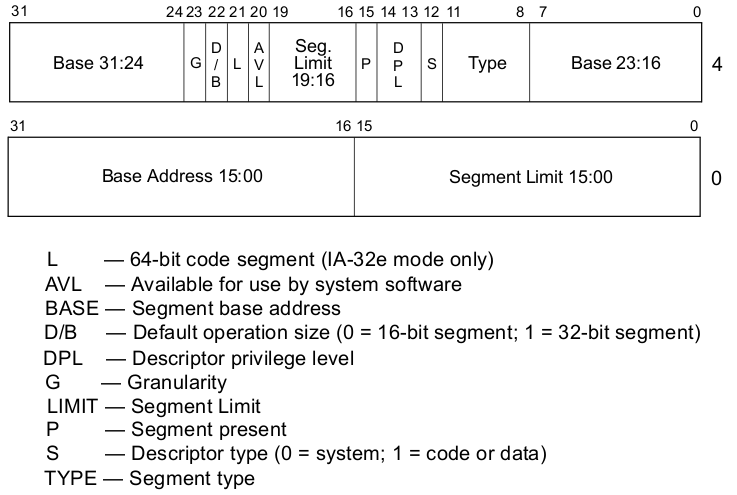
\includegraphics[width=\textwidth]{segment-descr}
};
%\draw[help lines] (0,0) grid (12, -8);
\begin{visibleenv}<2>
\draw[draw=red] (0.6, -5.4) rectangle (5.8, -5.8) node[right,text=red] {
    user or kernel mode? (if code)
};
\end{visibleenv}
\begin{visibleenv}<3>
\draw[draw=red] (0.6, -3.9) rectangle (8.0, -4.3);
\draw[draw=red] (0.6, -5.0) rectangle (11.0, -5.4);
\node[draw=red,text=red!60!black,anchor=north] at (5.0, -5.6) {
    64-bit or 32-bit or 16-bit mode? (if code)
};
\end{visibleenv}
\end{tikzpicture}
\imagecredit{Figure: Intel manuals, Volume 3A}
\end{frame}


\begin{frame}{64-bit segmentation}
\begin{itemize}
\item in 64-bit mode:
\item limits are ignored
\item base addresses are ignored
\item \ldots except for {\tt \%fs}, {\tt \%gs}
    \begin{itemize}
    \item when explicit segment override is used
    \end{itemize}
\item effectively: extra pointer register
\end{itemize}
\end{frame}

\begin{frame}[fragile,label=segAndRE]{segmentation and RE assignment}
\begin{lstlisting}
mov %fs:0x28, %rax
\end{lstlisting}
\end{frame}

\section{executable formats}

\begin{frame}{memory v. disk}
\begin{tikzpicture}
\tikzset{
    mylabel/.style={font=\ttfamily},
    mybox/.style={draw,rectangle,minimum width=5cm,fill=white},
    myboxD/.style={draw,rectangle,minimum width=6cm,fill=white},
    myhigh/.style={draw,rectangle,line width=1mm, draw=blue!80!black,opacity=.3},
    nomem/.style={black!50,draw=black,fill=white},
}
\node[mybox,minimum height=1cm,pattern=north west lines,pattern color=black!20!white] (kernel) {Used by OS};
\node[above=.2cm of kernel] {(virtual) memory};
\node[mybox, minimum height=.5cm, below=1cm of kernel] (stack) {Stack};
\node[mybox, minimum height=.5cm, below=1cm of stack] (heap) {Heap / other dynamic};
\node[mybox, minimum height=.5cm, below=0mm of heap] (data) {Writable data};
\node[mybox, minimum height=.5cm, below=0mm of data] (sdata) {Code + Constants};
\coordinate (memBottom) at ($(sdata.south east) + (0mm, -2mm)$);
\begin{pgfonlayer}{bg}
\draw[pattern=north west lines, pattern color=black!40!white] (kernel.north west) rectangle (memBottom);
\end{pgfonlayer}

\node[myboxD,below right=.5cm and 1cm of kernel,nomem] (diskHeader) {program header};
\node[above=.2cm of diskHeader] {program on disk};
\node[myboxD,below=0cm of diskHeader] (textSeg) { {\tt .text} (code) };
\node[myboxD,below=0cm of textSeg] (rodataSeg) { {\tt .rodata} (read-only data) };
\node[myboxD,below=0cm of rodataSeg] (dataSeg) { {\tt .data} };
\node[myboxD,below=0cm of dataSeg,pattern=north west lines, pattern color=black!40] (bssSeg) { {\tt .bss} (zeroes; not stored) };
.

\foreach \f/\t in {textSeg/sdata,rodataSeg/sdata,dataSeg/data,bssSeg/data} {
    \draw[thick,-Latex,black] (\f.west) -- (\t.east);
}
\end{tikzpicture}

% FIXME: add animation: binary file format
\end{frame}

\begin{frame}{ELF (executable and linking format)}
\begin{itemize}
\item Linux {\small (and some others)} executable/object file format
\end{itemize}
\begin{tikzpicture}
\tikzset{
    mybox/.style={draw,rectangle,minimum width=10cm,fill=white},
}
\node[mybox] (header) {
    \textbf{header}: machine type, file type, etc.
};
\node[mybox,below=0mm of header,align=center] (pHeader) {
    \textbf{program header}: ``\myemph{segments}'' to load \\
        (also, some other information)
};
\node[mybox,below=0mm of pHeader,align=center] (seg1) {
    \textbf{segment 1 data}
};
\node[mybox,below=0mm of seg1,align=center] (seg2) {
    \textbf{segment 2 data}
};
\node[mybox,below=3mm of seg2,align=center] (seg2) {
    \textbf{section header}:  \\ list of ``\myemph{sections}''(mostly for linker)
};
\end{tikzpicture}
\end{frame}

\begin{frame}{segments versus sections?}
\begin{itemize}
    \item note: ELF terminology; may not be true elsewhere!
    \item sections --- \myemph{object files} {\small (and usually executables)}, used by \myemph{linker}
        \begin{itemize}
        \item have information on intended purpose
        \item linkers combine these to create executables
        \item linkers might omit unneeded sections
        \end{itemize}
    \item segments --- executables, used to actually load program
        \begin{itemize}
        \item program loader is \myemph{dumb} --- doesn't know what segments are for
        \end{itemize}
\end{itemize}
\end{frame}

\subsection{static ELF example}
\newcommand{\myemphTwo}[1]{\myemph<2>{#1}}
\newcommand{\myemphTwoB}[1]{\myemph<2>{\textbf<2>{#1}}}
\newcommand{\myemphThree}[1]{\myemph<3>{#1}}
\newcommand{\myemphFour}[1]{\myemph<4>{#1}}
\newcommand{\myemphFive}[1]{\myemph<5>{#1}}
\newcommand{\myemphSix}[1]{\myemph<6>{#1}}
\newcommand{\myemphSeven}[1]{\myemph<7>{#1}}

\begin{frame}[fragile,label=elfExOver1]{ELF example}
    \begin{itemize}
    \item {\tt objdump -x /bin/busybox} (on my laptop)
    \item {\tt -x}: output all headers
    \end{itemize}
\begin{Verbatim}[commandchars=\\\{\},fontsize=\small]
/bin/busybox:     file format \myemphTwo{elf64-x86-64}
/bin/busybox
architecture: i386:x86-64, flags 0x00000102:
EXEC_P, D_PAGED
start address \myemphThree{0x0000000000401750}

Program Header:
[...]

Sections:
[...]
\end{Verbatim}
\end{frame}

\begin{frame}[fragile,label=elfExOver2]{a program header (1)}
\begin{Verbatim}[commandchars=\\\{\},fontsize=\fontsize{9}{10}\selectfont]
Program Header:
[...]
LOAD off    0x0000000 vaddr 0x0400000 paddr 0x0400000 align 2**21
     filesz 0x0\myemphTwo{1db697} memsz 0x01db697 flags \myemphThree{r-x}
LOAD off    0x01dbea8 vaddr 0x07dbea8 paddr 0x07dbea8 align 2**21
     filesz 0x000\myemphFour{21ee} memsz 0x000\myemphFour{7d18} flags rw-
[...]
\end{Verbatim}
\begin{itemize}
\item load {\tt \myemph<2>{0x1db697}} bytes:
        \begin{itemize}
        \item from {\tt 0x0} bytes into the file 
        \item to memory at {\tt 0x40000} \\
        \item \myemph<3>{readable and executable}
        \end{itemize}
\item load {\tt 0x21ee} bytes:
        \begin{itemize}
        \item from {\tt 0x1dbea8} 
        \item to memory at {\tt 0x7dbea8} 
        \item \myemph<4>{plus ({\tt 0x7d18}--{\tt 0x21ee}) bytes of zeroes}
        \item readable and writable
        \end{itemize}
\end{itemize}
\end{frame}

\begin{frame}[fragile,label=elfExOver3]{a program header (2)}
\begin{Verbatim}[commandchars=\\\{\},fontsize=\fontsize{9}{10}\selectfont]
Program Header:
[...]
 NOTE off    0x0000190 vaddr 0x0400190 paddr 0x0400190 align 2**2
      filesz 0x0000044 memsz 0x0000044 flags r--
  TLS  off    0x01dbea8 vaddr 0x07dbea8 paddr 0x07dbea8 align 2**3
      filesz 0x0000030 memsz 0x000007a flags r--
STACK off    0x0000000 vaddr 0x0000000 paddr 0x0000000 align 2**4
      filesz 0x0000000 memsz 0x0000000 flags rw-
RELRO off    0x01dbea8 vaddr 0x07dbea8 paddr 0x07dbea8 align 2**0
      filesz 0x0000158 memsz 0x0000158 flags r--
[...]
\end{Verbatim}
\begin{itemize}
\item NOTE --- comment
\item TLS --- thread-local storage region (used via {\tt \%fs})
\item STACK --- indicates stack is read/write
\item RELRO --- make this read-only after runtime linking
\end{itemize}
\end{frame}

\subsection{sections}

\begin{frame}[fragile,label=sectHeader]{section headers}
\vspace{-.25cm}
\begin{Verbatim}[fontsize=\tiny]
Sections:
Idx Name          Size      VMA               LMA               File off  Algn
  0 .note.ABI-tag 00000020  0000000000400190  0000000000400190  00000190  2**2
                  CONTENTS, ALLOC, LOAD, READONLY, DATA
  1 .note.gnu.build-id 00000024  00000000004001b0  00000000004001b0  000001b0  2**2
                  CONTENTS, ALLOC, LOAD, READONLY, DATA
  2 .rela.plt     00000210  00000000004001d8  00000000004001d8  000001d8  2**3
                  CONTENTS, ALLOC, LOAD, READONLY, DATA
  3 .init         0000001a  00000000004003e8  00000000004003e8  000003e8  2**2
                  CONTENTS, ALLOC, LOAD, READONLY, CODE
  4 .plt          00000160  0000000000400410  0000000000400410  00000410  2**4
                  CONTENTS, ALLOC, LOAD, READONLY, CODE
  5 .text         0017ff1d  0000000000400570  0000000000400570  00000570  2**4
                  CONTENTS, ALLOC, LOAD, READONLY, CODE
  6 __libc_freeres_fn 00002032  0000000000580490  0000000000580490  00180490  2**4
                  CONTENTS, ALLOC, LOAD, READONLY, CODE
  7 __libc_thread_freeres_fn 0000021b  00000000005824d0  00000000005824d0  001824d0  2**4
                  CONTENTS, ALLOC, LOAD, READONLY, CODE
  8 .fini         00000009  00000000005826ec  00000000005826ec  001826ec  2**2
                  CONTENTS, ALLOC, LOAD, READONLY, CODE
  9 .rodata       00044ac8  0000000000582700  0000000000582700  00182700  2**6
                  CONTENTS, ALLOC, LOAD, READONLY, DATA
 10 __libc_subfreeres 000000c0  00000000005c71c8  00000000005c71c8  001c71c8  2**3
                  CONTENTS, ALLOC, LOAD, READONLY, DATA
 11 .stapsdt.base 00000001  00000000005c7288  00000000005c7288  001c7288  2**0
                  CONTENTS, ALLOC, LOAD, READONLY, DATA
 12 __libc_atexit 00000008  00000000005c7290  00000000005c7290  001c7290  2**3
                  CONTENTS, ALLOC, LOAD, READONLY, DATA
 13 __libc_thread_subfreeres 00000018  00000000005c7298  00000000005c7298  001c7298  2**3
                  CONTENTS, ALLOC, LOAD, READONLY, DATA
 14 .eh_frame     000141dc  00000000005c72b0  00000000005c72b0  001c72b0  2**3
                  CONTENTS, ALLOC, LOAD, READONLY, DATA
 15 .gcc_except_table 0000020b  00000000005db48c  00000000005db48c  001db48c  2**0
                  CONTENTS, ALLOC, LOAD, READONLY, DATA
 16 .tdata        00000030  00000000007dbea8  00000000007dbea8  001dbea8  2**3
                  CONTENTS, ALLOC, LOAD, DATA, THREAD_LOCAL
 17 .tbss         0000004a  00000000007dbed8  00000000007dbed8  001dbed8  2**3
                  ALLOC, THREAD_LOCAL
 18 .init_array   00000010  00000000007dbed8  00000000007dbed8  001dbed8  2**3
                  CONTENTS, ALLOC, LOAD, DATA
 19 .fini_array   00000010  00000000007dbee8  00000000007dbee8  001dbee8  2**3
                  CONTENTS, ALLOC, LOAD, DATA
 20 .jcr          00000008  00000000007dbef8  00000000007dbef8  001dbef8  2**3
                  CONTENTS, ALLOC, LOAD, DATA
 21 .data.rel.ro  000000e8  00000000007dbf00  00000000007dbf00  001dbf00  2**6
                  CONTENTS, ALLOC, LOAD, DATA
 22 .got          00000010  00000000007dbfe8  00000000007dbfe8  001dbfe8  2**3
                  CONTENTS, ALLOC, LOAD, DATA
 23 .got.plt      000000c8  00000000007dc000  00000000007dc000  001dc000  2**3
                  CONTENTS, ALLOC, LOAD, DATA
 24 .data         00001f96  00000000007dc100  00000000007dc100  001dc100  2**6
                  CONTENTS, ALLOC, LOAD, DATA
 25 .bss          00005a90  00000000007de0c0  00000000007de0c0  001de096  2**6
                  ALLOC
 26 __libc_freeres_ptrs 00000070  00000000007e3b50  00000000007e3b50  001de096  2**3
                  ALLOC
 27 .note.stapsdt 0000100c  0000000000000000  0000000000000000  001de098  2**2
                  CONTENTS, READONLY
 28 .gnu_debuglink 00000034  0000000000000000  0000000000000000  001df0a4  2**0
                  CONTENTS, READONLY
\end{Verbatim}
\end{frame}

\begin{frame}{sections}
\begin{itemize}
\item tons of ``sections''
\item not actually needed/used to run program
\item size, file offset, flags (code/data/etc.)
    \begin{itemize}
    \item location in executable \textit{and} in memory
    \end{itemize}
\item some sections aren't stored (no ``CONTENTS'' flag) 
    \begin{itemize}
    \item just all zeroes
    \end{itemize}
\end{itemize}
\end{frame}

\begin{frame}{selected sections}
\begin{tabular}{rl}
    {\tt .text} & program code \\
    {\tt .bss} & initially zero data {\scriptsize (block started by symbol)} \\
    {\tt .data} & other writeable data  \\
    {\tt .rodata} & read-only data \\
    {\tt .init}/{\tt .fini} & global constructors/destructors \\
    {\tt .got}/{\tt .plt} & linking related \\
    {\tt .eh\_frame} & try/catch related \\
\end{tabular}
\imagecredit{based on \url{http://people.redhat.com/mpolacek/src/devconf2012.pdf}}
\end{frame}


\begin{frame}{other executable formats}
    \begin{itemize}
    \item PE (Portable Executable) --- Windows
    \item Mach-O --- MacOS X
    \item broadly similar to ELF
    \item differences:  
        \begin{itemize}
        \item whether segment/section distinction exists
        \item how linking/debugging info represented
        \item how program start info represented
        \end{itemize}
    \end{itemize}
\end{frame}


\section{executable startup}

\begin{frame}{simple executable startup}
    \begin{itemize}
    \item copy segments into memory
    \item jump to start address
    \end{itemize}
\end{frame}

\begin{frame}{executable startup code}
    \begin{itemize}
    \item Linux: executables don't start at {\tt main}
    \item why not?
        \begin{itemize}
        \item need to initialize {\tt printf}, {\tt cout}, {\tt malloc}, etc. data structures
        \item {\tt main} needs to return somewhere
        \end{itemize}
    \item compiler links in startup code
    \end{itemize}
\end{frame}

\subsection{relocations and symbol tables}

\section{dynamic linking primer}

\begin{frame}{linking}
    \begin{tikzpicture}
    \node[draw,font=\tt,very thick] (theCall) {callq printf};
    \node[draw,font=\tt,below=5cm of theCall,very thick] (theCallResolved) {callq 0x458F0};
    \draw[very thick,-Latex] (theCall) -- (theCallResolved);
    \end{tikzpicture}
\end{frame}

\begin{frame}{static v. dynamic linking}
    \begin{itemize}
    \item static linking --- linking \myemph{to create executable}
    \item dynamic linking --- linking \myemph{when executable is run}
    \vspace{.5cm}
    \item<2> conceptually: no difference in how they work
    \item<2> reality --- very different mechanisms
    \end{itemize}
\end{frame}

\begin{frame}{linking data structures}
    \begin{itemize}
    \item symbol table: {\tt name} $\Rightarrow$ (section, offset)
        \begin{itemize}
        \item example: {\tt main:} in assembly adds symbol table entry for {\tt main}
        \end{itemize}
    \item relocation table: offset $\Rightarrow$ (name, kind)
        \begin{itemize}
        \item example: {\tt call printf} adds relocation for name {\tt printf}
        \item kind depends on how instruction encodes address
        \end{itemize}
    \end{itemize}
\end{frame}

\begin{frame}[fragile,label=linkingExAsm]{hello.s}
\begin{lstlisting}
.data
string: .asciz "Hello, World!"
.text
.globl main
main:
    movq $string, %rdi
    call puts
    ret
\end{lstlisting}
\end{frame}

\begin{frame}[fragile,label=linkingExObj]{hello.o}
\begin{Verbatim}[commandchars=\\\{\},fontsize=\fontsize{9}{10}\selectfont]
SYMBOL TABLE:
0000000000000000 l    d  .text  0000000000000000 .text
0000000000000000 l    d  .data  0000000000000000 .data
0000000000000000 l    d  .bss   0000000000000000 .bss
0000000000000000 l       .data  0000000000000000 string
0000000000000000 \myemphSix{g}       \myemphSeven{.text  0000000000000000} main
0000000000000000         \myemphTwo{*UND*  0000000000000000 puts}

RELOCATION RECORDS FOR [.text]:
OFFSET           TYPE              VALUE 
0000000000000003 \myemphFive{R_X86_64_32S}      \myemphFour{.data}
0000000000000008 \myemphFive{R_X86_64_PC32}     \myemphThree{puts}-0x0000000000000004
\end{Verbatim}
\begin{tikzpicture}[overlay,remember picture]
    \tikzset{overBox/.style={at=(boxLoc),anchor=center,align=center,draw,rectangle,fill=white}}
    \coordinate (boxLoc) at ([yshift=-2.5cm]current page.center);
    \begin{visibleenv}<2>
        \node[overBox] {
            undefined symbol: look for {\tt puts} elsewhere
        };
    \end{visibleenv}
    \begin{visibleenv}<3>
        \node[overBox] {
           insert address of puts, format for {\tt call}
        };
    \end{visibleenv}
    \begin{visibleenv}<4>
        \node[overBox] {
           insert address of string, format for {\tt movq}
        };
    \end{visibleenv}
    \begin{visibleenv}<5>
        \node[overBox] {
            different ways to represent address \\
            {\tt 32S} --- signed 32-bit value \\
            {\tt PC32} --- 32-bit difference from current address
        };
    \end{visibleenv}
    \begin{visibleenv}<6>
        \node[overBox] {
            {\tt g}: global --- used by other files \\
            {\tt l}: local 
        };
    \end{visibleenv}
    \begin{visibleenv}<7>
        \node[overBox] {
            {\tt .text} segment beginning plus 0 bytes
        };
    \end{visibleenv}
\end{tikzpicture}
\end{frame}

\begin{frame}{interlude: strace}
\begin{itemize}
\item {\tt strace} --- system call tracer
    \begin{itemize}
    \item on Linux, some other Unices
    \item OS X approx. equivalent: {\tt dtruss}
    \item Windows approx. equivalent: Process Monitor
    \end{itemize}
\item indicates what system calls (operating system services) used by a program
\end{itemize}
\end{frame}

\begin{frame}[fragile,label=staticStrace]{statically linked hello.exe}
\begin{itemize}
\item \small{\tt gcc -static -o hello-static.exe hello.s}
\item \small{\tt strace ./hello-static.exe}:
\end{itemize}
\begin{Verbatim}[commandchars=@\{\},fontsize=\fontsize{8}{9}\selectfont]
execve("./hello-static.exe", ["./hello-static.exe"], [/* 46 vars */]) = 0
@myemphTwo{uname({sysname="Linux", nodename="reiss-lenovo", ...}) = 0}
@myemphTwo{brk(NULL)                               = 0x20a5000}
@myemphThree{brk(0x20a61c0)                          = 0x20a61c0}
@myemphTwo{arch_prctl(ARCH_SET_FS, 0x20a5880)      = 0}
@myemphTwo{readlink("/proc/self/exe", "/home/cr4bd/spring2017/cs4630/sl"..., 4096) = 62}
@myemphThree{brk(0x20c71c0)                          = 0x20c71c0}
@myemphThree{brk(0x20c8000)                          = 0x20c8000}
@myemphTwo{access("/etc/ld.so.nohwcap", F_OK)}      = -1 ENOENT (No such file or directory)
@myemphFour{fstat(1, {st_mode=S_IFCHR|0620, st_rdev=makedev(136, 1), ...}) = 0}
@myemphFour{write(1, "Hello, World!\n", 14)         = 14}
@myemphFive{exit_group(14)}                          = ?
+++ exited with 14 +++
\end{Verbatim}
\begin{tikzpicture}[overlay,remember picture]
    \tikzset{
        overBoxGeneric/.style={
            anchor=center,
            align=center,
            draw,
            rectangle,
            fill=white,
            draw=red!70!black,very thick},
        overBox/.style={
            overBoxGeneric,
            at=(boxLoc),
        },
        overBoxB/.style={
            overBoxGeneric,
            at=(boxLocB),
        },
    }
    \coordinate (boxLoc) at ([yshift=-3.5cm]current page.center);
    \begin{visibleenv}<2>
        \node[overBox] {
            standard library startup
        };
    \end{visibleenv}
    \begin{visibleenv}<3>
        \node[overBox] {
            memory allocation
        };
    \end{visibleenv}
    \begin{visibleenv}<4>
        \node[overBox] {
            implementation of puts
        };
    \end{visibleenv}
    \begin{visibleenv}<5>
        \node[overBox] {
            standard library shutdown
        };
    \end{visibleenv}
\end{tikzpicture}
\end{frame}

\begin{frame}[fragile,label=straceDynamic]{dynamically linked hello.exe}
\begin{itemize}
\item \small{\tt gcc -o hello.exe hello.s}
\item \small{\tt strace ./hello.exe}:
\end{itemize}
\begin{Verbatim}[commandchars=@\{\},fontsize=\fontsize{8}{9}\selectfont]
execve("./hello.exe", ["./hello.exe"], [/* 46 vars */]) = 0
@textit{...}
@myemphThree{mmap(NULL, 8192, PROT_READ|PROT_WRITE, MAP_PRIVATE|MAP_ANONYMOUS, -1, 0)} = 0x7fdfeeb39000
access("/etc/ld.so.preload", R_OK)      = -1 ENOENT (No such file or directory)
open("/etc/ld.so.cache", O_RDONLY|O_CLOEXEC) = 3
fstat(3, {st_mode=S_IFREG|0644, st_size=137808, ...}) = 0
@textit{...}
open("@myemphTwoB{/lib/x86_64-linux-gnu/libc.so.6}", O_RDONLY|O_CLOEXEC) = 3
@myemphFour{read(3, "\177ELF\2\1\1\3\0\0\0\0\0\0\0\0\3\0>\0\1\0\0\0P\t\2\0\0\0\0\0"..., 832) = 832}
fstat(3, {st_mode=S_IFREG|0755, st_size=1864888, ...}) = 0
@myemphFive{mmap(NULL, 3967392, PROT_READ|PROT_EXEC, ..., 3, 0) = 0x7fdfee54d000}
mprotect(0x7fdfee70c000, 2097152, PROT_NONE) = 0
@myemphFive{mmap(0x7fdfee90c000, 24576, PROT_READ|PROT_WRITE, ..., 3, 0x1bf000) = 0x7fdfee90c000}
@myemphSix{mmap(0x7fdfee912000, 14752, PROT_READ|PROT_WRITE, ..., -1, 0) = 0x7fdfee912000}
close(3)                                = 0
@textit{...}
write(1, "Hello, World!\n", 14)         = 14
exit_group(14)                          = ?
+++ exited with 14 +++
\end{Verbatim}
\begin{tikzpicture}[overlay,remember picture]
    \tikzset{overBox/.style={at=(boxLoc),anchor=center,align=center,draw,rectangle,fill=white,draw=red!70!black,very thick}}
    \coordinate (boxLoc) at (current page.center);
    \begin{visibleenv}<2>
        \node[overBox] {
            the standard C library (includes {\texttt{puts}}
        };
    \end{visibleenv}
    \begin{visibleenv}<3>
        \node[overBox] {
            memory allocation (different method)
        };
    \end{visibleenv}
    \begin{visibleenv}<4>
        \node[overBox] {
            read standard C library header
        };
    \end{visibleenv}
    \begin{visibleenv}<5>
        \node[overBox] {
            load standard C library ({\tt 3} = opened file)
        };
    \end{visibleenv}
    \begin{visibleenv}<6>
        \node[overBox] {
            allocate zero-initialized data segment for C library
        };
    \end{visibleenv}
\end{tikzpicture}
\end{frame}

\begin{frame}{dynamic linking}
\begin{itemize}
    \item load and link (find address of {\tt puts}) \myemph{runtime}
    \item advantages:
        \begin{itemize}
        \item smaller executables
        \item easier upgrades
        \item less memory usage (load one copy of library for multiple programs)
        \end{itemize}
    \item disadvantages:
        \begin{itemize}
        \item library upgrades breaking programs
        \item programs less compatible between OS versions
        \item possibly slower
        \end{itemize}
\end{itemize}
\end{frame}

\begin{frame}{where's the linker}
\begin{itemize}
    \item Where's the code that calls {\tt open("...libc.so.6")}?
    \item Could check {\tt hello.exe} --- it's not there!
    \vspace{.5cm}
    \item<2> instead: ``interpreter'' {\tt /lib64/ld-linux-x86-64.so.2}
    \item<2> on Linux: contains loading code instead of core OS
        \begin{itemize}
        \item OS loads it instead of program
        \end{itemize}
\end{itemize}
\end{frame}

\begin{frame}[fragile,label=interpObjdump]{objdump --- the interpreter}
\begin{itemize}
\item excerpt from {\tt objdump -sx hello.exe}:
\end{itemize}
\begin{Verbatim}[commandchars=@\{\},fontsize=\fontsize{8}{9}\selectfont]
Program Header:
@textit{...}
  INTERP off    0x0000238 vaddr 0x0@myemph{400238} paddr 0x0400238 align 2**0
         filesz 0x000001c memsz 0x000001c flags r--
@textit{...}
Contents of section .interp:
 @myemph{400238} 2f6c6962 36342f6c 642d6c69 6e75782d  @myemph{/lib64/ld-linux-}
 400248 7838362d 36342e73 6f2e3200           @myemph{x86-64.so.2}.    
\end{Verbatim}
\end{frame}

\begin{frame}{dynamic linking information}
\begin{itemize}
\item \myemph{symbol table} --- works the same, but in executable
\item could use same relocations --- but these are \myemph{expensive}
\item rather just copy data from disk without changes
\item solutions: global lookup table!
\end{itemize}
\end{frame}

\begin{frame}[fragile,label=dynamicPuts]{dynamically linked puts}
\begin{Verbatim}[commandchars=Q\{\},fontsize=\fontsize{8}{9}\selectfont]
0000000000400400 <puts@plt>:
  400400:	ff 25 12 0c 20 00    	jmpq   *0x200c12(%rip) 
                    /* 0x200c12+RIP = _GLOBAL_OFFSET_TABLE_+0x18 */
Qtextit{... later in main: ...}
  40052d:	e8 ce fe ff ff       	callq  400400 <puts@plt>
                        /* instead of call puts */
\end{Verbatim}
\begin{itemize}
    \item replace {\tt puts} with \myemph{stub} {\tt puts@plt} 
        \begin{itemize}
        \item plt = procedure linkage table
        \end{itemize}
    \item stub: jump to {\tt *\_GLOBAL\_OFFSET\_TABLE[3]}
    \item dynamic linker changes \myemph{table instead of code}
        \begin{itemize}
        \item could change code --- just would be less efficient
        \end{itemize}
\end{itemize}
\end{frame}

\begin{frame}[fragile,label=dynamicPutsLazy]{lazy binding}
\begin{Verbatim}[commandchars=Q\{\},fontsize=\fontsize{8}{9}\selectfont]
0000000000400400 <puts@plt>:
  400400:	ff 25 12 0c 20 00    	jmpq   *0x200c12(%rip) 
                    /* 0x200c12+RIP = _GLOBAL_OFFSET_TABLE_+0x18 */
  400406:	68 00 00 00 00       	pushq  $0x0
  40040b:	e9 e0 ff ff ff       	jmpq   4003f0 <_init+0x28>
\end{Verbatim}
\begin{itemize}
    \item could fill global offset table immediately
    \item alternative: fill on demand
    \item extra code ({\tt pushq} then {\tt jmpq}) runs ``fixup code''
        \begin{itemize}
        \item reads symbol tables to find function
        \item edits global offset table
        \item jumps to function
        \end{itemize}
    \item called ``lazy binding''
\end{itemize}
\end{frame}

\begin{frame}{lazy binding pro/con}
\begin{itemize}
    \item advantages:
    \begin{itemize}
        \item faster program loading
        \item no overhead for unused code (often a lot of stuff)
    \end{itemize}
    \item disadvantages:
    \begin{itemize}
        \item can move errors (missing functions, etc.) to runtime
        \item possibly more total overhead
    \end{itemize}
\end{itemize}
\end{frame}




\section{x86-64 instruction encoding}

\begin{frame}{x86 instruction encoding}
\begin{itemize}
    \item in 2110, 3330 you learned a ``teaching'' machine code
    \item Y86 (3330) is very like what x86 should be
    \item \ldots but it isn't
    \item why? history!
\end{itemize}
\end{frame}

\begin{frame}{the 8086}
\begin{tikzpicture}[overlay,remember picture]
\node[anchor=north east] {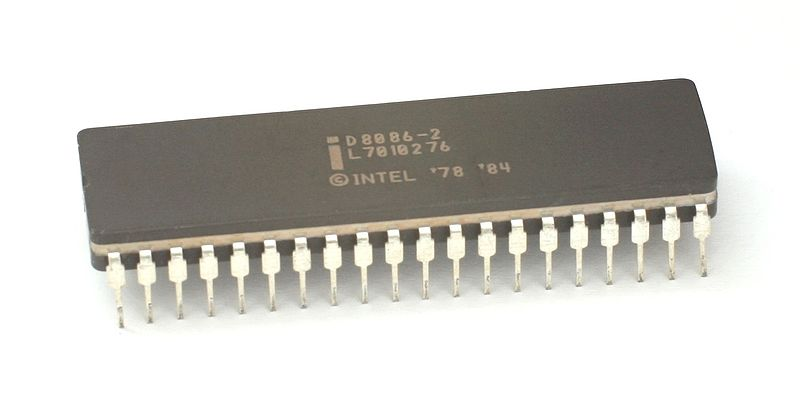
\includegraphics[width=0.3\textwidth]{Intel8086}};
\end{tikzpicture}
\begin{itemize}
    \item 1979 Intel processor
    \item 4 general purpose 16-bit registers: AX, BX, CX, DX
    \item 4 special 16-bit registers: SI, DI, BP, SP
\end{itemize}
\end{frame}

\begin{frame}{8086 instruction encoding: simple}
\begin{itemize}
    \item special cases: 1-byte instructions:
    \begin{itemize}
    \item anything with no arguments
    \item push ax, push bx, push cx, \ldots (dedicated opcodes)
    \item pop ax, \ldots
    \end{itemize}
\end{itemize}
\end{frame}

\begin{frame}{8086 instruction encoding: two-arg}
\begin{itemize}
    \item 1-byte opcode
    \item sometimes {\tt ModRM} byte:
        \begin{itemize}
        \item 2-bit ``mod'' and 
        \item 3-bit register number (source or dest, depends on opcode) and
        \item 3-bit ``r/m''
        \end{itemize}
    \item ``mod'' + ``r/m'' specify one of:
        \begin{itemize}
        \item {\tt \%reg} (mod = {\tt 11})
        \item {\tt (\%bx/\%bp, \%si/\%di)}
        \item {\tt (\%bx/\%si/\%di)}
        \item {\tt offset(\%bx/\%bp/,\%si/\%di)} (8- or 16-byte offset)
        \end{itemize}
    \item non-intuitive table
\end{itemize}
\end{frame}

\begin{frame}{8086 ModRM table}
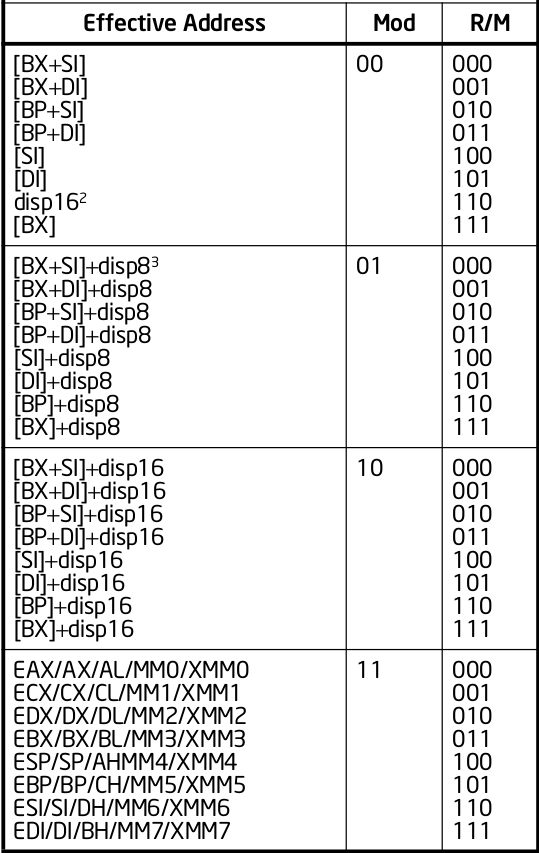
\includegraphics[height=0.8\textheight]{16bitmodrm}
\end{frame}

\begin{frame}{8086 evolution}
\begin{itemize}
\item Intel 8086 --- 1979, 16-bit registers
\item Intel (80)386 --- 1986, 32-bit registers
\item AMD K8 --- 2003, 64-bit registers
\end{itemize}
\end{frame}

\begin{frame}{x86 modes}
\begin{itemize}
\item x86 has multiple \myemph{modes}
\item maintains compatiblity
\item e.g.: modern x86 processor can work like 8086
    \begin{itemize}
    \item called ``real mode''
    \end{itemize}
\item different mode for 32-bit/64-bit
\item same basic encoding; some sizes change
\end{itemize}
\end{frame}

\begin{frame}{32-bit ModRM table}
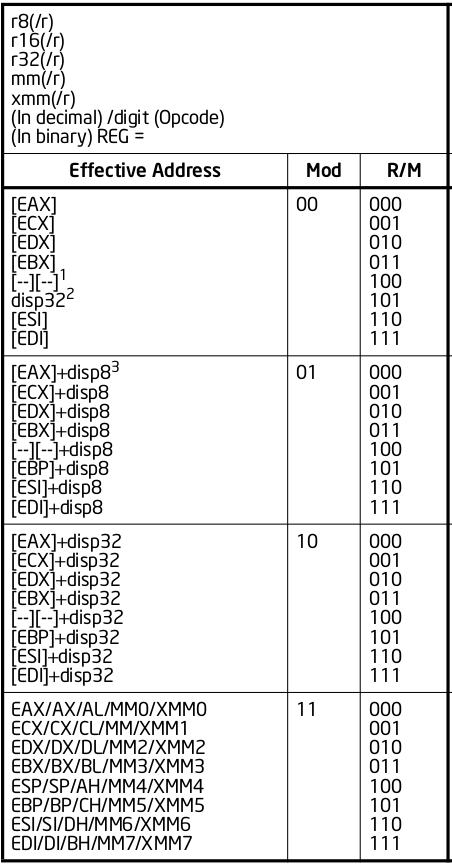
\includegraphics[height=0.8\textheight]{32bitmodrm}
\end{frame}

\begin{frame}{32-bit addition: SIB bytes}
\begin{itemize}
\item 8086 addressing modes made registers different
\item 32-bit mode got rid of this (mostly)
\item problem: not enough spare bits in {\tt ModRM} byte
\item solution: if ``r/m'' bits = {\tt 100}, extra ``SIB'' byte:
    \begin{itemize}
    \item 2 bit \myemph<2>{scale}: {\tt 00} is 1, {\tt 01} is 2, {\tt 10} is 4, {\tt 11} is 8
    \item 3 bit \myemph<3>{index}: index register number
    \item 3 bit \myemph<4>{base}: base register number
    \end{itemize}
\item {\tt (\myemph<4>{\%baseReg},\myemph<3>{\%indexReg},\myemph<2>{scale})}
\end{itemize}
\end{frame}

\begin{frame}{intel manual: SIB table}
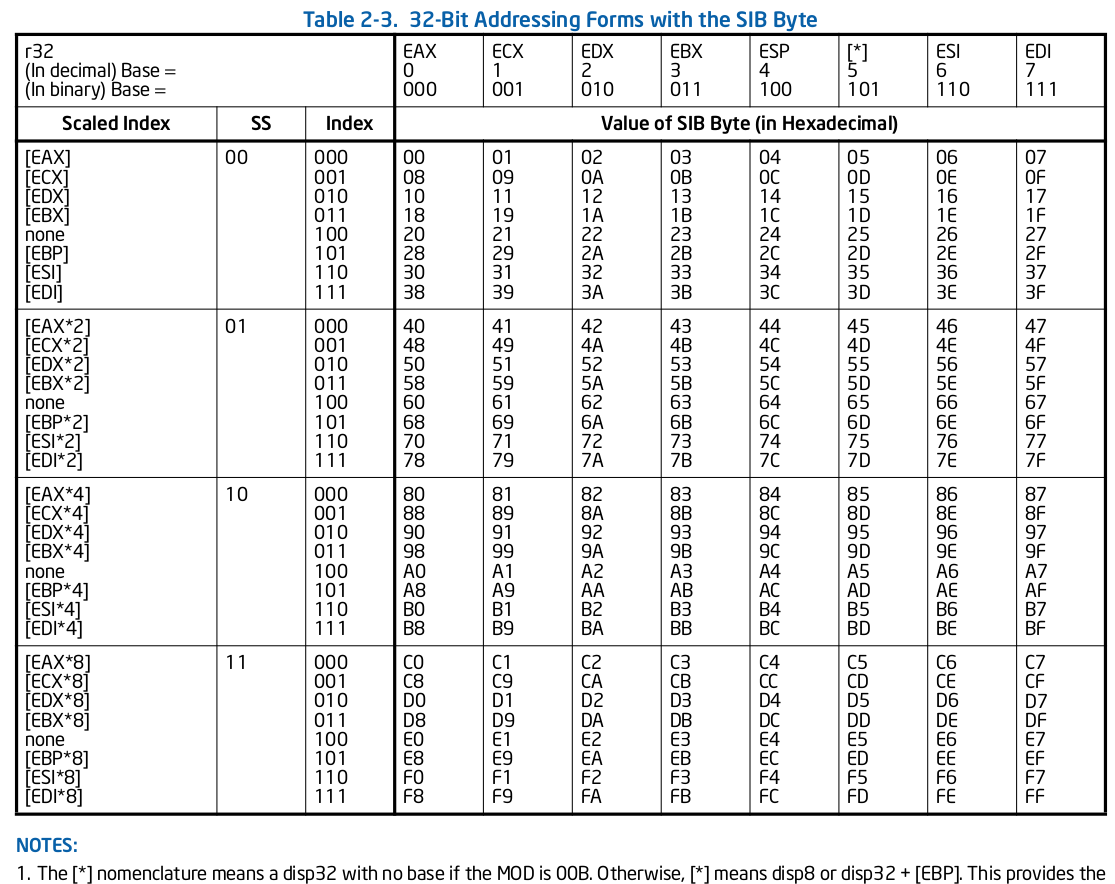
\includegraphics[height=0.8\textheight]{32bitsib}
\end{frame}

\begin{frame}{basic 32-bit encoding}
\begin{tikzpicture}
\begin{scope}[start chain=going right,node distance=0mm,every node/.style={on chain,draw,font=\small,minimum height=1cm}]
\node { opcode }; \node[dashed] { ModRM byte}; \node[dashed] {SIB byte}; \node[dashed] {displacement}; \node[dashed] {immediate};
\end{scope}
\end{tikzpicture}
\begin{itemize}
\item dashed: not always present
\item opcodes: 1-3 bytes
    \begin{itemize}
    \item some 5-bit opcodes, with 3-bit register field
    \item (alternate view: 8-bit opcode with fixed register)
    \item sometimes part of ModRM used as add'tl part of opcode
    \end{itemize}
\item displacement, immediate: 1, 2, or 4 bytes
    \begin{itemize}
    \item or, rarely, 8 bytes
    \end{itemize}
\end{itemize}
\end{frame}

\begin{frame}{what about 64-bit?}
\begin{itemize}
\item adds 8 more registers --- more bits for reg \#?
\item didn't change encoding for existing instructions, so\ldots
\item \myemph{instruction prefix} ``REX''
    \begin{itemize}
    \item 32-bit x86 already had many prefixes
    \end{itemize}
\item also selects 64-bit version of instruction
\end{itemize}
\end{frame}

\begin{frame}{REX prefix}
\begin{tikzpicture}
    \node[draw,rectangle split,rectangle split horizontal, rectangle split parts=5,
        label={north:REX prefix byte}] (rexbyte) {
        {\tt 0100}
        \nodepart{two}
        w
        \nodepart{three}
        r
        \nodepart{four}
        s
        \nodepart{five}
        b
    };
    \node[anchor=north west,align=left] (wExplain) at ([yshift=-5cm,xshift=.5cm]rexbyte.five south) {
        {\tt 1} if 64-bit regs ({\tt \%rax}, etc.)\\
        {\tt 0} if 32-bit regs ({\tt \%eax}, etc.)
    };
    \draw[thick,-Latex] (rexbyte.two south) |- (wExplain.west);
    \node[anchor=south west] (rExplain) at ([yshift=1mm]wExplain.north west) {
        extra bit for ModRM reg field
    };
    \draw[thick,-Latex] (rexbyte.three south) |- (rExplain.west);
    \node[anchor=south west] (sExplain) at ([yshift=1mm]rExplain.north west) {
        extra bit for SIB byte index reg field
    };
    \draw[thick,-Latex] (rexbyte.four south) |- (sExplain.west);
    \node[anchor=south west, align=left] (bExplain) at ([yshift=1mm]sExplain.north west) {
        extra bit for ModRM r/m \\ or SIB base reg field
    };
    \draw[thick,-Latex] (rexbyte.five south) |- (bExplain.west);
\end{tikzpicture}
%\vspace{.5cm}
%\item 4-bit constant 0100
%\item 1-bit ``w'': 1 if 64-bit operands
%\item 1-bit ``r'': extra bit for ModRM register number
%\item 1-bit ``s'': extra bit for SIB index register number
%\item 1-bit ``b'': extra bit for ``r/m'' or SIB index register number 
%    \begin{itemize}
%    \item or modify in-opcode register number
%    \end{itemize}
%\end{itemize}
\end{frame}

\begin{frame}{overall encoding}
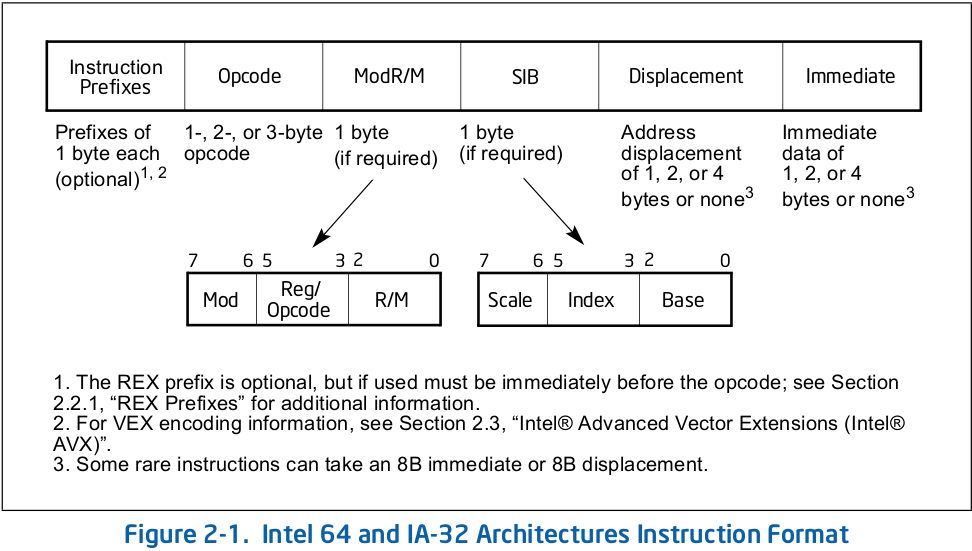
\includegraphics[width=\textwidth]{IntelFig21}
\end{frame}

\begin{frame}<1>[label=prefixes]{instruction prefixes}
    \begin{itemize}
    \item REX (64-bit and/or extra register bits)
    \item VEX (SSE/AVX instructions; other new instrs.)
    \item operand/address-size change (64/32 to 16 or vice-versa)
    \item {\tt LOCK} --- synchronization between processors
    \item \myemph<2>{{\tt REPNE/REPNZ/REP/REPE/REPZ} --- turns instruction into loop}
    \item segment overrides
    \end{itemize}
\end{frame}

\begin{frame}[fragile,label=x86ex1]{x86 encoding example (1)}
    \begin{itemize}
    \item \lstinline|pushq %rax| encoded as {\tt 50}
        \begin{itemize}
        \item 5-bit opcode {\tt 01010} plus 3-bit register number {\tt 000}
        \end{itemize}
    \item \lstinline|pushq %r13| encoded as {\tt 41 55}
        \begin{itemize}
        \item {\tt 41}: REX prefix {\tt 0010} (constant), w:{\tt 0}, r:{\tt 0}, s:{\tt 0}, b:{\tt \color{blue!80!black}{1}}
        \item w = {\tt 0} because push is never 32-bit in 64-bit mode
        \item {\tt 55}: 5-bit opcode {\tt 01010}; 3-bit reg \# {\tt \color{green!80!black}{101}}
        \item 4-bit reg \# {\tt \color{blue!80!black}{1}\color{green!80!black}{101}} = 13
        \end{itemize}
    \end{itemize}
\end{frame}

\begin{frame}[fragile,label=x86ex2]{x86 encoding example (2)}
    \begin{itemize}
    \item \lstinline|addq 0x12345678(%rax,%rbx,2), %ecx|
    \item {\tt 03}: opcode --- add r/m32 to r/m32
    \item {\tt 8c}: ModRM: mod = {\tt 10}; reg = {\tt 001}, r/m: {\tt 100}
        \begin{itemize}
        \item reg = {\tt 001} = {\tt \%ecx} (table)
        \item SIB byte + 32-bit displacement (table)
        \end{itemize}
    \item {\tt 58}: SIB: scale = {\tt 01}, index = {\tt 011}, base = {\tt 000}
        \begin{itemize}
        \item index {\tt 011} = {\tt \%rbx}; base {\tt 000} = {\tt \%rax};
        \end{itemize}
    \item {\tt 78 56 32 12}: 32-bit constant {\tt 0x12345678}
    \end{itemize}
\end{frame}

\begin{frame}[fragile,label=x86ex3]{x86 encoding example (3)}
    \begin{itemize}
    \item \lstinline|addq 0x12345678(%r10,%r11,2), %rax|
    \item {\tt 4b}: REX prefix {\tt 0100}+w:{\tt \myemph<2>{1}}, r:{\tt \textcolor{orange!80!black}{0}}, s:{\tt \textcolor{blue!80!black}{1}}, b:{\tt \textcolor{green!80!black}{1}}
    \item {\tt 03}: opcode --- add r/m64 to r64 (with \myemph<2>{REX.w})
    \item {\tt 84}: ModRM: mod = {\tt 10}; reg = {\tt 000}, r/m: {\tt 100}
        \begin{itemize}
        \item reg = {\tt \textcolor{orange!80!black}{0}000} = \%rax
        \item SIB byte + 32-bit displacement (table)
        \end{itemize}
    \item {\tt 5a}: SIB: scale = {\tt 01}, index = {\tt 011}, base = {\tt 010}
        \begin{itemize}
        \item with REX: index = {\tt \textcolor{blue!80!black}{1}011} (11), base = {\tt \textcolor{green!80!black}{1}010} (10)
        \end{itemize}
    \item {\tt 78 56 32 12}: 32-bit constant {\tt 0x12345678}
    \end{itemize}
\end{frame}

\begin{frame}[fragile,label=x86ex4]{x86 encoding example (4)}
    \begin{itemize}
    \item \lstinline|movq %fs:0x10,%r13|
    \item {\tt 64}: FS segment override
    \item {\tt 48}: REX: {\tt w}: 1 (64-bit), {\tt r}: \textcolor{orange!80!black}{1}, {\tt s}: \textcolor{blue!80!black}{0}, {\tt b}: \textcolor{green!80!black}{0}
    \item {\tt 8b}: opcode for MOV memory to register
    \item {\tt 2c}: ModRM: mod = {\tt 00}, reg = {\tt 101}, r/m: {\tt 100}
        \begin{itemize}
        \item with REX: reg = {\tt \textbf{\textcolor{orange!80!black}{1}}101} [\%r12]; r/m = {100} (SIB follows)
        \end{itemize}
    \item {\tt 25}: SIB: scale = {\tt 00}; index = {\tt \textcolor{blue!80!black}{0}100}; base = {\tt \textcolor{green!80!black}{0}101}
        \begin{itemize}
        \item no register/no register in table
        \end{itemize}
    \item {\tt 10 00 00 00}: 4-byte constant {\tt 0x10}
    \end{itemize}
\end{frame}

\begin{frame}[fragile,label=x8664impos]{x86-64 impossibilities}
\lstset{
    language=myasm,
    style=small,
    moredelim={**[is][\sout<all:1>]{~sout~}{~endsout~}},
}
    \begin{itemize}
    \item \myemph{illegal}: \lstinline|~sout~movq 0x12345678ab(%rax), %rax~endsout~|
        \begin{itemize}
        \item maximum 32-bit displacement
        \item \lstinline|movq 0x12345678ab, %rax| okay
            \begin{itemize}
            \item extra {\tt mov} opcode for {\tt \%rax} only
            \end{itemize}
        \end{itemize}
    \item \myemph{illegal}: \lstinline|~sout~movq $0x12345678ab, %rbx~endsout~|
        \begin{itemize}
        \item maximum 32-bit constant
        \item \lstinline|movq $0x12345678ab, %rax| okay
        \end{itemize}
    \item \myemph{illegal}: \lstinline|~sout~pushl %eax~endsout~|
        \begin{itemize}
        \item no 32-bit push/pop in 64-bit mode
        \item but 16-bit allowed (operand size prefix byte {\tt 66})
        \end{itemize}
    \item \myemph{illegal}: \lstinline|~sout~movq (%rax, %rsp), %rax~endsout~|
        \begin{itemize}
        \item cannot use \lstinline|%rsp| as index register
        \item \lstinline|movq (%rsp, %rax), %rax| okay
        \end{itemize}
    \end{itemize}
\end{frame}

\againframe<2>{prefixes}

\begin{frame}[fragile,label=string1]{string instructions (1)}
\begin{lstlisting}[style=small]
memcpy: // copy %rdx bytes from (%rsi) to (%rdi)
        cmpq %rdx, %rdx
        je done
        movsb
        subq $1, %rdx
        jmp memcpy
done:   ret
\end{lstlisting}
\begin{itemize}
\item {\tt movsb} (move data from string to string, byte)
\item mov one byte from {\tt (\%rsi)} to {\tt (\%rdi)}
\item increment \%rsi and \%rdi (*)
\item \myemph{cannot} specify other registers
\end{itemize}
\end{frame}

\begin{frame}[fragile,label=string2]{string instructions (2)}
\begin{lstlisting}[style=small]
memcpy: // copy %rdx bytes from (%rsi) to (%rdi)
    rep movsb
    ret
\end{lstlisting}
\begin{itemize}
\item {\tt rep} prefix byte
\vspace{.5cm}
\item repeat instruction until {\tt \%rdx} is 0
\item decrement {\tt \%rdx} each time
\item \myemph{cannot} specify other registers
\item \myemph{cannot} use {\tt rep} with all instructions
\end{itemize}
\end{frame}

\begin{frame}{string instructions (3)}
\begin{itemize}
\item {\tt lodsb}, {\tt stosb} --- load/store into string
\item {\tt movsw}, {\tt movsd} --- word/dword versions
\item string comparison instructions
\vspace{.5cm}
\item {\tt rep movsb} is still recommended on modern Intel
    \begin{itemize}
    \item special-cased in processor?
    \end{itemize}
\end{itemize}
\end{frame}

% FIXME: more examples?

\section{a note on assembly and optimization}

\begin{frame}{exploring assembly}
\begin{itemize}
\item compiling little C programs looking at the assembly is nice:
\item {\tt gcc -S \myemph<2>{\textbf<2>{-O}}}
    \begin{itemize}
    \item extra stuff like {\tt .cfi} directives (for try/catch)
    \end{itemize}
\vspace{.5cm}
\item or disassemble:
\item {\tt gcc \myemph<2>{\textbf<2>{-O}} -c file.c} (or make an executable)
\item {\tt objdump -dr file.o} (or on an executable) 
    \begin{itemize}
    \item d: disassemble
    \item r: show (non-dynamic) relocations
    \end{itemize}
\end{itemize}
\end{frame}

\begin{frame}[fragile,label=noOpt]{assembly without optimizations}
\begin{itemize}
\item compilers do \myemph{really silly things} without optimizations:
\begin{lstlisting}[language=C, style=smaller]
int sum(int x, int y) { return x + y; }
\end{lstlisting}
\vspace{-.125cm}
\begin{lstlisting}[language=myasm,style=smaller]
sum:
    pushq   %rbp
    movq    %rsp, %rbp
    movl    %edi, -4(%rbp)
    movl    %esi, -8(%rbp)
    movl    -4(%rbp), %edx
    movl    -8(%rbp), %eax
    addl    %edx, %eax
    popq    %rbp
    ret
\end{lstlisting}
\vspace{-.3cm}
\item instead of {\tt gcc -O} version:
\vspace{-.1cm}
\begin{lstlisting}[language=myasm,style=smaller]
sum:
    leal (%rdi,%rsi), %eax
    ret
\end{lstlisting}
\end{itemize}
\end{frame}

\section{more resources}

\section{looking at assembly by hand}

\begin{frame}{assembly reading advice}
    \begin{itemize}
    \item don't know what an instruction does: look it up!
    \item remember calling conventions
    \item function/variable names (if present) help
    \item try to name values in registers, on stack
        \begin{itemize}
        \item based on context
        \item ``input size'' not ``rax''
        \end{itemize}
    \end{itemize}
\end{frame}

\begin{frame}{next time: looking at viruses}
    \begin{itemize}
    \item how/where to insert virus code?
    \item how/where to copy self?
    \end{itemize}
\end{frame}
